\section{Design of Architecture} \label{sec:overview}

We chose the Linux Kernel Virtual Machine (\kvm)~\cite{kivity2007kvm} as the 
platform of our study. \kvm takes advantage of the hardware virtualization 
extensions so that it achieves nearlythe same performance with the underlying 
physical machine. A major advantage of the \kvm architecture is the full 
availability of user-space tools in the \qemu process, such as threading, 
libraries and so on.

Figure~\ref{fig:arc} shows our proposed architecture in \kvm virtualization environment. 
Only the primary VM advertises its presence on the network, so all network 
inputs come to the primary VM. 

It contains three main components: the Serviceguard, a tailored version 
of \qemu, and the \smr system \smrsystem. 

The Serviceguard is deployed on the virtual machine, and provides monitoring 
capabilities for applications running inside virtual machines in the \kvm 
virtualization environment.

\begin{figure}[t]
% \vspace{.20in}
\centering
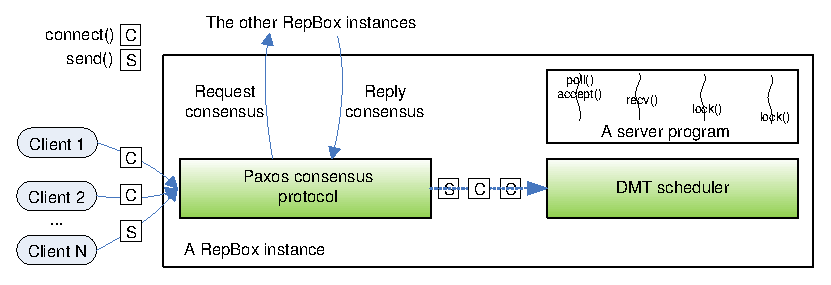
\includegraphics[width=.47\textwidth]{figures/arch}
\vspace{-.2in}
\caption{{\em Proposed architecture in \kvm virtualization environment.} Key 
components are shaded (and in blue).} \label{fig:arc}
\vspace{.05in}
\end{figure}
